\documentclass[1p]{elsarticle_modified}
%\bibliographystyle{elsarticle-num}

%\usepackage[colorlinks]{hyperref}
%\usepackage{abbrmath_seonhwa} %\Abb, \Ascr, \Acal ,\Abf, \Afrak
\usepackage{amsfonts}
\usepackage{amssymb}
\usepackage{amsmath}
\usepackage{amsthm}
\usepackage{scalefnt}
\usepackage{amsbsy}
\usepackage{kotex}
\usepackage{caption}
\usepackage{subfig}
\usepackage{color}
\usepackage{graphicx}
\usepackage{xcolor} %% white, black, red, green, blue, cyan, magenta, yellow
\usepackage{float}
\usepackage{setspace}
\usepackage{hyperref}

\usepackage{tikz}
\usetikzlibrary{arrows}

\usepackage{multirow}
\usepackage{array} % fixed length table
\usepackage{hhline}

%%%%%%%%%%%%%%%%%%%%%
\makeatletter
\renewcommand*\env@matrix[1][\arraystretch]{%
	\edef\arraystretch{#1}%
	\hskip -\arraycolsep
	\let\@ifnextchar\new@ifnextchar
	\array{*\c@MaxMatrixCols c}}
\makeatother %https://tex.stackexchange.com/questions/14071/how-can-i-increase-the-line-spacing-in-a-matrix
%%%%%%%%%%%%%%%

\usepackage[normalem]{ulem}

\newcommand{\msout}[1]{\ifmmode\text{\sout{\ensuremath{#1}}}\else\sout{#1}\fi}
%SOURCE: \msout is \stkout macro in https://tex.stackexchange.com/questions/20609/strikeout-in-math-mode

\newcommand{\cancel}[1]{
	\ifmmode
	{\color{red}\msout{#1}}
	\else
	{\color{red}\sout{#1}}
	\fi
}

\newcommand{\add}[1]{
	{\color{blue}\uwave{#1}}
}

\newcommand{\replace}[2]{
	\ifmmode
	{\color{red}\msout{#1}}{\color{blue}\uwave{#2}}
	\else
	{\color{red}\sout{#1}}{\color{blue}\uwave{#2}}
	\fi
}

\newcommand{\Sol}{\mathcal{S}} %segment
\newcommand{\D}{D} %diagram
\newcommand{\A}{\mathcal{A}} %arc


%%%%%%%%%%%%%%%%%%%%%%%%%%%%%5 test

\def\sl{\operatorname{\textup{SL}}(2,\Cbb)}
\def\psl{\operatorname{\textup{PSL}}(2,\Cbb)}
\def\quan{\mkern 1mu \triangleright \mkern 1mu}

\theoremstyle{definition}
\newtheorem{thm}{Theorem}[section]
\newtheorem{prop}[thm]{Proposition}
\newtheorem{lem}[thm]{Lemma}
\newtheorem{ques}[thm]{Question}
\newtheorem{cor}[thm]{Corollary}
\newtheorem{defn}[thm]{Definition}
\newtheorem{exam}[thm]{Example}
\newtheorem{rmk}[thm]{Remark}
\newtheorem{alg}[thm]{Algorithm}

\newcommand{\I}{\sqrt{-1}}
\begin{document}

%\begin{frontmatter}
%
%\title{Boundary parabolic representations of knots up to 8 crossings}
%
%%% Group authors per affiliation:
%\author{Yunhi Cho} 
%\address{Department of Mathematics, University of Seoul, Seoul, Korea}
%\ead{yhcho@uos.ac.kr}
%
%
%\author{Seonhwa Kim} %\fnref{s_kim}}
%\address{Center for Geometry and Physics, Institute for Basic Science, Pohang, 37673, Korea}
%\ead{ryeona17@ibs.re.kr}
%
%\author{Hyuk Kim}
%\address{Department of Mathematical Sciences, Seoul National University, Seoul 08826, Korea}
%\ead{hyukkim@snu.ac.kr}
%
%\author{Seokbeom Yoon}
%\address{Department of Mathematical Sciences, Seoul National University, Seoul, 08826,  Korea}
%\ead{sbyoon15@snu.ac.kr}
%
%\begin{abstract}
%We find all boundary parabolic representation of knots up to 8 crossings.
%
%\end{abstract}
%\begin{keyword}
%    \MSC[2010] 57M25 
%\end{keyword}
%
%\end{frontmatter}

%\linenumbers
%\tableofcontents
%
\newcommand\colored[1]{\textcolor{white}{\rule[-0.35ex]{0.8em}{1.4ex}}\kern-0.8em\color{red} #1}%
%\newcommand\colored[1]{\textcolor{white}{ #1}\kern-2.17ex	\textcolor{white}{ #1}\kern-1.81ex	\textcolor{white}{ #1}\kern-2.15ex\color{red}#1	}

{\Large $\underline{12a_{0589}~(K12a_{0589})}$}

\setlength{\tabcolsep}{10pt}
\renewcommand{\arraystretch}{1.6}
\vspace{1cm}\begin{tabular}{m{100pt}>{\centering\arraybackslash}m{274pt}}
\multirow{5}{120pt}{
	\centering
	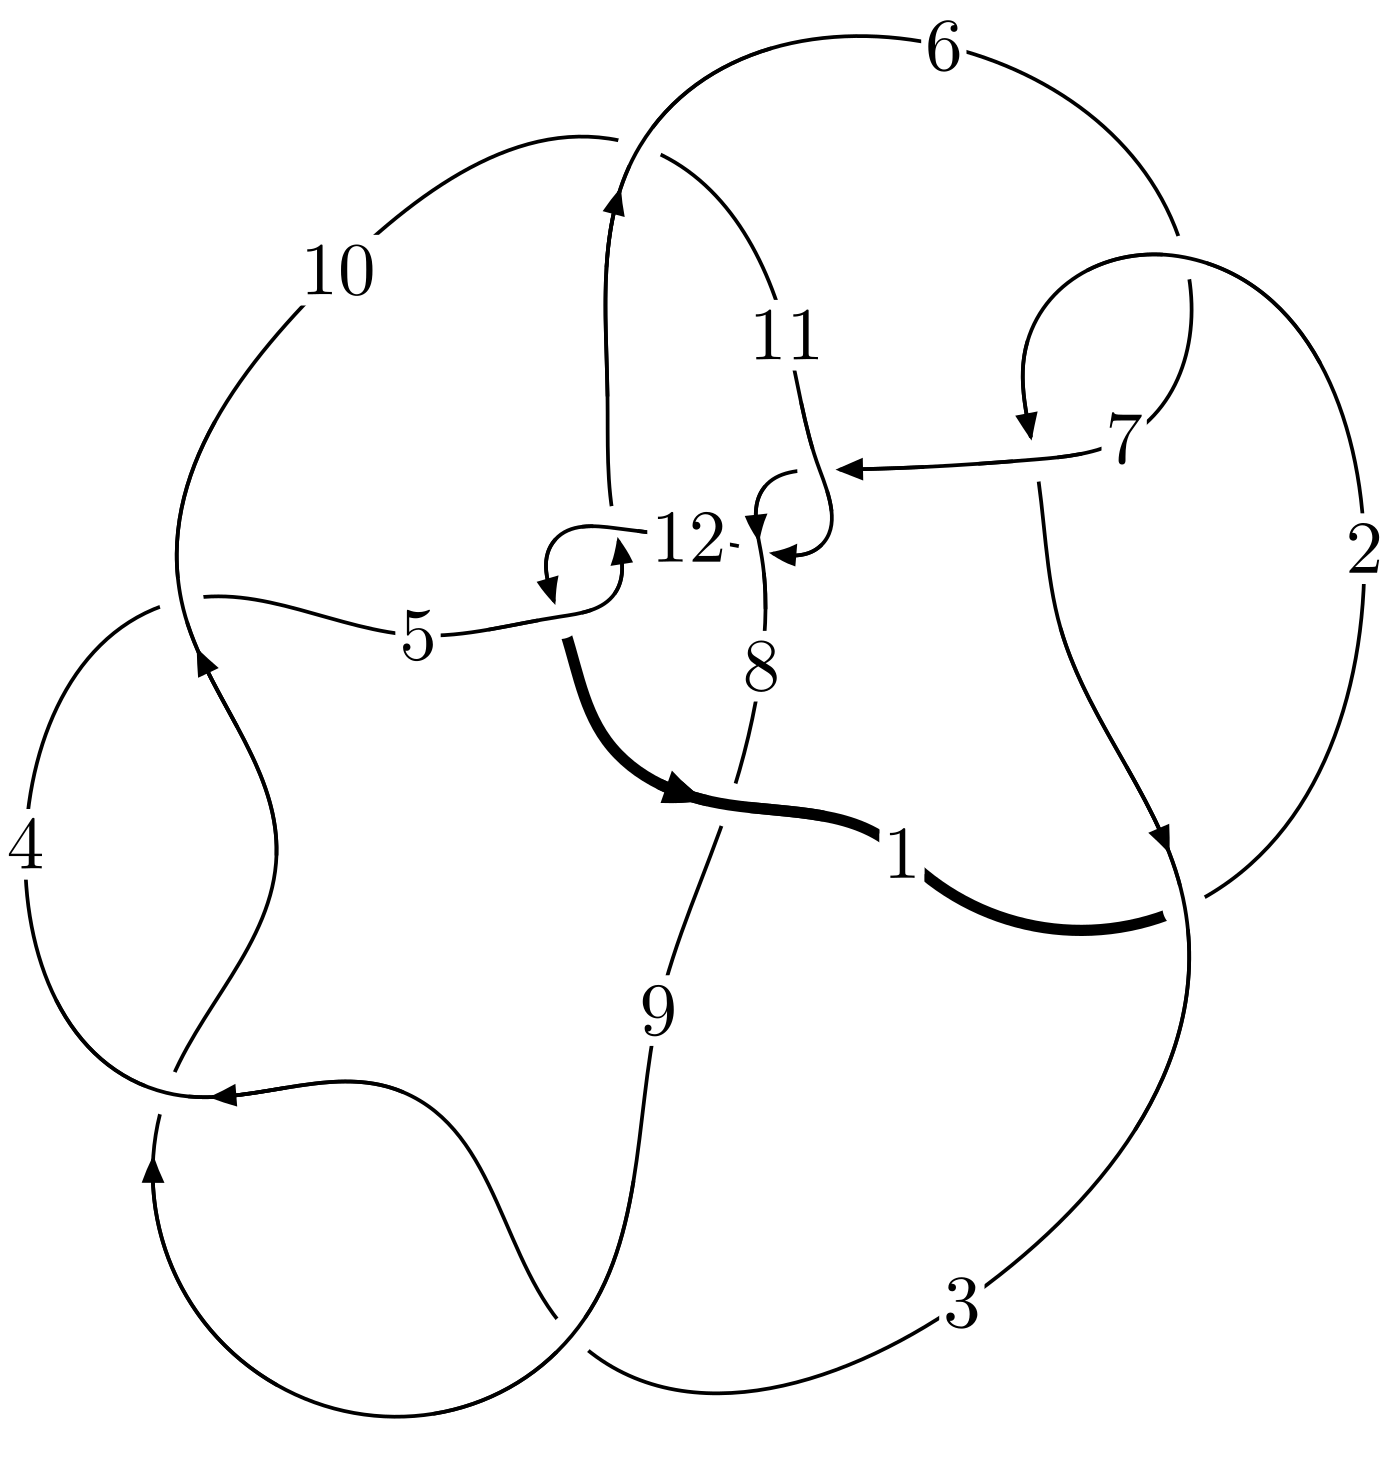
\includegraphics[width=112pt]{../../../GIT/diagram.site/Diagrams/png/1390_12a_0589.png}\\
\ \ \ A knot diagram\footnotemark}&
\allowdisplaybreaks
\textbf{Linearized knot diagam} \\
\cline{2-2}
 &
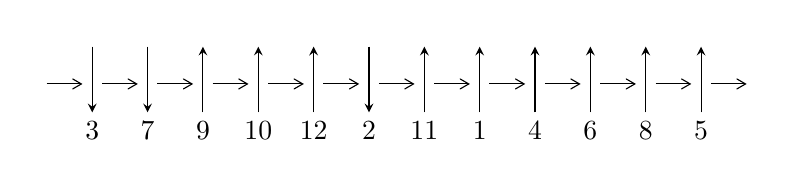
\begin{tikzpicture}[x=20pt, y=17pt]
	% nodes
	\node (C0) at (0, 0) {};
	\node (C1) at (1, 0) {};
	\node (C1U) at (1, +1) {};
	\node (C1D) at (1, -1) {3};

	\node (C2) at (2, 0) {};
	\node (C2U) at (2, +1) {};
	\node (C2D) at (2, -1) {7};

	\node (C3) at (3, 0) {};
	\node (C3U) at (3, +1) {};
	\node (C3D) at (3, -1) {9};

	\node (C4) at (4, 0) {};
	\node (C4U) at (4, +1) {};
	\node (C4D) at (4, -1) {10};

	\node (C5) at (5, 0) {};
	\node (C5U) at (5, +1) {};
	\node (C5D) at (5, -1) {12};

	\node (C6) at (6, 0) {};
	\node (C6U) at (6, +1) {};
	\node (C6D) at (6, -1) {2};

	\node (C7) at (7, 0) {};
	\node (C7U) at (7, +1) {};
	\node (C7D) at (7, -1) {11};

	\node (C8) at (8, 0) {};
	\node (C8U) at (8, +1) {};
	\node (C8D) at (8, -1) {1};

	\node (C9) at (9, 0) {};
	\node (C9U) at (9, +1) {};
	\node (C9D) at (9, -1) {4};

	\node (C10) at (10, 0) {};
	\node (C10U) at (10, +1) {};
	\node (C10D) at (10, -1) {6};

	\node (C11) at (11, 0) {};
	\node (C11U) at (11, +1) {};
	\node (C11D) at (11, -1) {8};

	\node (C12) at (12, 0) {};
	\node (C12U) at (12, +1) {};
	\node (C12D) at (12, -1) {5};
	\node (C13) at (13, 0) {};

	% arrows
	\draw[->,>={angle 60}]
	(C0) edge (C1) (C1) edge (C2) (C2) edge (C3) (C3) edge (C4) (C4) edge (C5) (C5) edge (C6) (C6) edge (C7) (C7) edge (C8) (C8) edge (C9) (C9) edge (C10) (C10) edge (C11) (C11) edge (C12) (C12) edge (C13) ;	\draw[->,>=stealth]
	(C1U) edge (C1D) (C2U) edge (C2D) (C3D) edge (C3U) (C4D) edge (C4U) (C5D) edge (C5U) (C6U) edge (C6D) (C7D) edge (C7U) (C8D) edge (C8U) (C9D) edge (C9U) (C10D) edge (C10U) (C11D) edge (C11U) (C12D) edge (C12U) ;
	\end{tikzpicture} \\
\hhline{~~} \\& 
\textbf{Solving Sequence} \\ \cline{2-2} 
 &
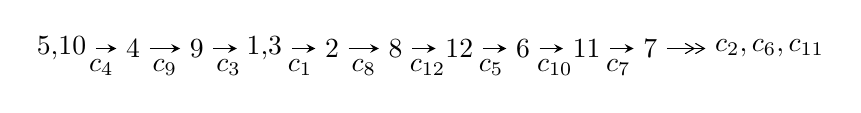
\begin{tikzpicture}[x=23pt, y=7pt]
	% node
	\node (A0) at (-1/8, 0) {5,10};
	\node (A1) at (1, 0) {4};
	\node (A2) at (2, 0) {9};
	\node (A3) at (49/16, 0) {1,3};
	\node (A4) at (33/8, 0) {2};
	\node (A5) at (41/8, 0) {8};
	\node (A6) at (49/8, 0) {12};
	\node (A7) at (57/8, 0) {6};
	\node (A8) at (65/8, 0) {11};
	\node (A9) at (73/8, 0) {7};
	\node (C1) at (1/2, -1) {$c_{4}$};
	\node (C2) at (3/2, -1) {$c_{9}$};
	\node (C3) at (5/2, -1) {$c_{3}$};
	\node (C4) at (29/8, -1) {$c_{1}$};
	\node (C5) at (37/8, -1) {$c_{8}$};
	\node (C6) at (45/8, -1) {$c_{12}$};
	\node (C7) at (53/8, -1) {$c_{5}$};
	\node (C8) at (61/8, -1) {$c_{10}$};
	\node (C9) at (69/8, -1) {$c_{7}$};
	\node (A10) at (11, 0) {$c_{2},c_{6},c_{11}$};

	% edge
	\draw[->,>=stealth]	
	(A0) edge (A1) (A1) edge (A2) (A2) edge (A3) (A3) edge (A4) (A4) edge (A5) (A5) edge (A6) (A6) edge (A7) (A7) edge (A8) (A8) edge (A9) ;
	\draw[->>,>={angle 60}]	
	(A9) edge (A10);
\end{tikzpicture} \\ 

\end{tabular} \\

\footnotetext{
The image of knot diagram is generated by the software ``\textbf{Draw programme}" developed by Andrew Bartholomew(\url{http://www.layer8.co.uk/maths/draw/index.htm\#Running-draw}), where we modified some parts for our purpose(\url{https://github.com/CATsTAILs/LinksPainter}).
}\phantom \\ \newline 
\centering \textbf{Ideals for irreducible components\footnotemark of $X_{\text{par}}$} 
 
\begin{align*}
I^u_{1}&=\langle 
-7.11582\times10^{221} u^{99}-8.63174\times10^{221} u^{98}+\cdots+1.62343\times10^{221} b-3.59350\times10^{222},\\
\phantom{I^u_{1}}&\phantom{= \langle  }-4.74270\times10^{224} u^{99}-5.73839\times10^{224} u^{98}+\cdots+3.73389\times10^{222} a-2.20342\times10^{225},\\
\phantom{I^u_{1}}&\phantom{= \langle  }u^{100}+u^{99}+\cdots+14 u-1\rangle \\
I^u_{2}&=\langle 
u^3+b,\;- u^3+2 u^2+3 a+2 u-1,\;u^4- u^2+1\rangle \\
I^u_{3}&=\langle 
u^3+b,\;- u^3- u^2+3 a+2 u-1,\;u^4- u^2+1\rangle \\
\\
\end{align*}
\raggedright * 3 irreducible components of $\dim_{\mathbb{C}}=0$, with total 108 representations.\\
\footnotetext{All coefficients of polynomials are rational numbers. But the coefficients are sometimes approximated in decimal forms when there is not enough margin.}
\newpage
\renewcommand{\arraystretch}{1}
\centering \section*{I. $I^u_{1}= \langle -7.12\times10^{221} u^{99}-8.63\times10^{221} u^{98}+\cdots+1.62\times10^{221} b-3.59\times10^{222},\;-4.74\times10^{224} u^{99}-5.74\times10^{224} u^{98}+\cdots+3.73\times10^{222} a-2.20\times10^{225},\;u^{100}+u^{99}+\cdots+14 u-1 \rangle$}
\flushleft \textbf{(i) Arc colorings}\\
\begin{tabular}{m{7pt} m{180pt} m{7pt} m{180pt} }
\flushright $a_{5}=$&$\begin{pmatrix}1\\0\end{pmatrix}$ \\
\flushright $a_{10}=$&$\begin{pmatrix}0\\u\end{pmatrix}$ \\
\flushright $a_{4}=$&$\begin{pmatrix}1\\u^2\end{pmatrix}$ \\
\flushright $a_{9}=$&$\begin{pmatrix}- u\\- u^3+u\end{pmatrix}$ \\
\flushright $a_{1}=$&$\begin{pmatrix}127.018 u^{99}+153.684 u^{98}+\cdots-5600.34 u+590.115\\4.38320 u^{99}+5.31698 u^{98}+\cdots-199.270 u+22.1353\end{pmatrix}$ \\
\flushright $a_{3}=$&$\begin{pmatrix}- u^2+1\\- u^4+2 u^2\end{pmatrix}$ \\
\flushright $a_{2}=$&$\begin{pmatrix}133.223 u^{99}+161.070 u^{98}+\cdots-5878.58 u+619.701\\4.83883 u^{99}+5.87137 u^{98}+\cdots-222.047 u+24.6627\end{pmatrix}$ \\
\flushright $a_{8}=$&$\begin{pmatrix}508.169 u^{99}+596.373 u^{98}+\cdots-24295.6 u+2806.67\\7.84464 u^{99}+8.68358 u^{98}+\cdots-428.049 u+56.5824\end{pmatrix}$ \\
\flushright $a_{12}=$&$\begin{pmatrix}122.634 u^{99}+148.367 u^{98}+\cdots-5401.07 u+567.979\\4.38320 u^{99}+5.31698 u^{98}+\cdots-199.270 u+22.1353\end{pmatrix}$ \\
\flushright $a_{6}=$&$\begin{pmatrix}55.7325 u^{99}+63.3082 u^{98}+\cdots-2893.42 u+361.738\\0.770246 u^{99}+1.01289 u^{98}+\cdots-36.2687 u+5.09196\end{pmatrix}$ \\
\flushright $a_{11}=$&$\begin{pmatrix}621.926 u^{99}+735.391 u^{98}+\cdots-29150.1 u+3301.04\\12.8285 u^{99}+14.6903 u^{98}+\cdots-658.830 u+81.8685\end{pmatrix}$ \\
\flushright $a_{7}=$&$\begin{pmatrix}-96.2686 u^{99}-119.321 u^{98}+\cdots+3938.19 u-382.399\\-6.04319 u^{99}-7.28700 u^{98}+\cdots+275.012 u-29.1983\end{pmatrix}$\\&\end{tabular}
\flushleft \textbf{(ii) Obstruction class $= -1$}\\~\\
\flushleft \textbf{(iii) Cusp Shapes $= -4.33253 u^{99}-12.0749 u^{98}+\cdots-581.309 u+160.926$}\\~\\
\newpage\renewcommand{\arraystretch}{1}
\flushleft \textbf{(iv) u-Polynomials at the component}\newline \\
\begin{tabular}{m{50pt}|m{274pt}}
Crossings & \hspace{64pt}u-Polynomials at each crossing \\
\hline $$\begin{aligned}c_{1}\end{aligned}$$&$\begin{aligned}
&u^{100}+35 u^{99}+\cdots+5314 u+169
\end{aligned}$\\
\hline $$\begin{aligned}c_{2},c_{6}\end{aligned}$$&$\begin{aligned}
&u^{100}-3 u^{99}+\cdots-20 u+13
\end{aligned}$\\
\hline $$\begin{aligned}c_{3},c_{4},c_{9}\end{aligned}$$&$\begin{aligned}
&u^{100}- u^{99}+\cdots-14 u-1
\end{aligned}$\\
\hline $$\begin{aligned}c_{5},c_{12}\end{aligned}$$&$\begin{aligned}
&u^{100}-3 u^{99}+\cdots-128 u+52
\end{aligned}$\\
\hline $$\begin{aligned}c_{7},c_{11}\end{aligned}$$&$\begin{aligned}
&u^{100}-5 u^{99}+\cdots+22 u-1
\end{aligned}$\\
\hline $$\begin{aligned}c_{8}\end{aligned}$$&$\begin{aligned}
&529(529 u^{100}+2323 u^{99}+\cdots-5.59128\times10^{7} u-3.11681\times10^{7})
\end{aligned}$\\
\hline $$\begin{aligned}c_{10}\end{aligned}$$&$\begin{aligned}
&529(529 u^{100}+3841 u^{99}+\cdots+8995520 u-970300)
\end{aligned}$\\
\hline
\end{tabular}\\~\\
\newpage\renewcommand{\arraystretch}{1}
\flushleft \textbf{(v) Riley Polynomials at the component}\newline \\
\begin{tabular}{m{50pt}|m{274pt}}
Crossings & \hspace{64pt}Riley Polynomials at each crossing \\
\hline $$\begin{aligned}c_{1}\end{aligned}$$&$\begin{aligned}
&y^{100}+65 y^{99}+\cdots-6927358 y+28561
\end{aligned}$\\
\hline $$\begin{aligned}c_{2},c_{6}\end{aligned}$$&$\begin{aligned}
&y^{100}-35 y^{99}+\cdots-5314 y+169
\end{aligned}$\\
\hline $$\begin{aligned}c_{3},c_{4},c_{9}\end{aligned}$$&$\begin{aligned}
&y^{100}-95 y^{99}+\cdots-58 y+1
\end{aligned}$\\
\hline $$\begin{aligned}c_{5},c_{12}\end{aligned}$$&$\begin{aligned}
&y^{100}+53 y^{99}+\cdots-89080 y+2704
\end{aligned}$\\
\hline $$\begin{aligned}c_{7},c_{11}\end{aligned}$$&$\begin{aligned}
&y^{100}-55 y^{99}+\cdots-82 y+1
\end{aligned}$\\
\hline $$\begin{aligned}c_{8}\end{aligned}$$&$\begin{aligned}
&279841(279841 y^{100}-5042957 y^{99}+\cdots-6.77314\times10^{16} y+9.71451\times10^{14})
\end{aligned}$\\
\hline $$\begin{aligned}c_{10}\end{aligned}$$&$\begin{aligned}
&279841\\
&\cdot(279841 y^{100}-18269015 y^{99}+\cdots-953537733200 y+941482090000)
\end{aligned}$\\
\hline
\end{tabular}\\~\\
\newpage\flushleft \textbf{(vi) Complex Volumes and Cusp Shapes}
$$\begin{array}{c|c|c}  
\text{Solutions to }I^u_{1}& \I (\text{vol} + \sqrt{-1}CS) & \text{Cusp shape}\\
 \hline 
\begin{aligned}
u &= \phantom{-}0.494564 + 0.868297 I \\
a &= \phantom{-}0.957136 - 0.711585 I \\
b &= \phantom{-}0.595137 + 1.233490 I\end{aligned}
 & \phantom{-}1.56718 + 13.70260 I & \phantom{-0.000000 } 0 \\ \hline\begin{aligned}
u &= \phantom{-}0.494564 - 0.868297 I \\
a &= \phantom{-}0.957136 + 0.711585 I \\
b &= \phantom{-}0.595137 - 1.233490 I\end{aligned}
 & \phantom{-}1.56718 - 13.70260 I & \phantom{-0.000000 } 0 \\ \hline\begin{aligned}
u &= -0.594360 + 0.794669 I \\
a &= -0.315966 - 0.050179 I \\
b &= \phantom{-}0.519602 + 1.007160 I\end{aligned}
 & \phantom{-}3.10737 + 2.58864 I & \phantom{-0.000000 } 0 \\ \hline\begin{aligned}
u &= -0.594360 - 0.794669 I \\
a &= -0.315966 + 0.050179 I \\
b &= \phantom{-}0.519602 - 1.007160 I\end{aligned}
 & \phantom{-}3.10737 - 2.58864 I & \phantom{-0.000000 } 0 \\ \hline\begin{aligned}
u &= \phantom{-}0.546169 + 0.879548 I \\
a &= -0.641283 + 0.597330 I \\
b &= -0.371361 - 0.967519 I\end{aligned}
 & -1.19926 + 1.95519 I & \phantom{-0.000000 } 0 \\ \hline\begin{aligned}
u &= \phantom{-}0.546169 - 0.879548 I \\
a &= -0.641283 - 0.597330 I \\
b &= -0.371361 + 0.967519 I\end{aligned}
 & -1.19926 - 1.95519 I & \phantom{-0.000000 } 0 \\ \hline\begin{aligned}
u &= -0.529573 + 0.783995 I \\
a &= -0.952631 - 0.685469 I \\
b &= -0.603749 + 1.220150 I\end{aligned}
 & \phantom{-}2.97162 - 7.84264 I & \phantom{-0.000000 } 0 \\ \hline\begin{aligned}
u &= -0.529573 - 0.783995 I \\
a &= -0.952631 + 0.685469 I \\
b &= -0.603749 - 1.220150 I\end{aligned}
 & \phantom{-}2.97162 + 7.84264 I & \phantom{-0.000000 } 0 \\ \hline\begin{aligned}
u &= -0.435240 + 0.977287 I \\
a &= \phantom{-}0.608130 + 0.654085 I \\
b &= \phantom{-}0.430468 - 1.039270 I\end{aligned}
 & -2.05758 - 7.06500 I & \phantom{-0.000000 } 0 \\ \hline\begin{aligned}
u &= -0.435240 - 0.977287 I \\
a &= \phantom{-}0.608130 - 0.654085 I \\
b &= \phantom{-}0.430468 + 1.039270 I\end{aligned}
 & -2.05758 + 7.06500 I & \phantom{-0.000000 } 0\\
 \hline 
 \end{array}$$\newpage$$\begin{array}{c|c|c}  
\text{Solutions to }I^u_{1}& \I (\text{vol} + \sqrt{-1}CS) & \text{Cusp shape}\\
 \hline 
\begin{aligned}
u &= \phantom{-}0.721353 + 0.811301 I \\
a &= \phantom{-}0.168237 + 0.016183 I \\
b &= -0.529096 + 1.067270 I\end{aligned}
 & \phantom{-}2.19181 - 8.06866 I & \phantom{-0.000000 } 0 \\ \hline\begin{aligned}
u &= \phantom{-}0.721353 - 0.811301 I \\
a &= \phantom{-}0.168237 - 0.016183 I \\
b &= -0.529096 - 1.067270 I\end{aligned}
 & \phantom{-}2.19181 + 8.06866 I & \phantom{-0.000000 } 0 \\ \hline\begin{aligned}
u &= \phantom{-}0.787367 + 0.395930 I \\
a &= \phantom{-}0.003217 + 0.657953 I \\
b &= -0.347285 + 1.118780 I\end{aligned}
 & -2.34706 - 2.72684 I & \phantom{-0.000000 } 0 \\ \hline\begin{aligned}
u &= \phantom{-}0.787367 - 0.395930 I \\
a &= \phantom{-}0.003217 - 0.657953 I \\
b &= -0.347285 - 1.118780 I\end{aligned}
 & -2.34706 + 2.72684 I & \phantom{-0.000000 } 0 \\ \hline\begin{aligned}
u &= -0.559331 + 0.641843 I \\
a &= \phantom{-}0.395096 + 0.141503 I \\
b &= \phantom{-}0.990205 + 0.205441 I\end{aligned}
 & \phantom{-}4.69005 - 8.03457 I & \phantom{-0.000000 } 0 \\ \hline\begin{aligned}
u &= -0.559331 - 0.641843 I \\
a &= \phantom{-}0.395096 - 0.141503 I \\
b &= \phantom{-}0.990205 - 0.205441 I\end{aligned}
 & \phantom{-}4.69005 + 8.03457 I & \phantom{-0.000000 } 0 \\ \hline\begin{aligned}
u &= \phantom{-}0.881092 + 0.739200 I \\
a &= -0.183885 + 0.313689 I \\
b &= \phantom{-}0.171550 - 0.635394 I\end{aligned}
 & -0.32711 + 3.86344 I & \phantom{-0.000000 } 0 \\ \hline\begin{aligned}
u &= \phantom{-}0.881092 - 0.739200 I \\
a &= -0.183885 - 0.313689 I \\
b &= \phantom{-}0.171550 + 0.635394 I\end{aligned}
 & -0.32711 - 3.86344 I & \phantom{-0.000000 } 0 \\ \hline\begin{aligned}
u &= -0.388057 + 0.754681 I \\
a &= -0.438833 - 1.099830 I \\
b &= -0.639728 + 0.405220 I\end{aligned}
 & \phantom{-}4.11149 + 3.49119 I & \phantom{-0.000000 } 0 \\ \hline\begin{aligned}
u &= -0.388057 - 0.754681 I \\
a &= -0.438833 + 1.099830 I \\
b &= -0.639728 - 0.405220 I\end{aligned}
 & \phantom{-}4.11149 - 3.49119 I & \phantom{-0.000000 } 0\\
 \hline 
 \end{array}$$\newpage$$\begin{array}{c|c|c}  
\text{Solutions to }I^u_{1}& \I (\text{vol} + \sqrt{-1}CS) & \text{Cusp shape}\\
 \hline 
\begin{aligned}
u &= \phantom{-}0.220257 + 0.785544 I \\
a &= \phantom{-}0.174053 - 1.140200 I \\
b &= \phantom{-}0.598970 + 0.513921 I\end{aligned}
 & \phantom{-}4.54056 + 1.86436 I & \phantom{-0.000000 } 0 \\ \hline\begin{aligned}
u &= \phantom{-}0.220257 - 0.785544 I \\
a &= \phantom{-}0.174053 + 1.140200 I \\
b &= \phantom{-}0.598970 - 0.513921 I\end{aligned}
 & \phantom{-}4.54056 - 1.86436 I & \phantom{-0.000000 } 0 \\ \hline\begin{aligned}
u &= -0.172179 + 0.766268 I \\
a &= \phantom{-}0.649580 + 0.848586 I \\
b &= \phantom{-}0.319532 - 1.179920 I\end{aligned}
 & -5.75809 - 1.64364 I & \phantom{-0.000000 } 0 \\ \hline\begin{aligned}
u &= -0.172179 - 0.766268 I \\
a &= \phantom{-}0.649580 - 0.848586 I \\
b &= \phantom{-}0.319532 + 1.179920 I\end{aligned}
 & -5.75809 + 1.64364 I & \phantom{-0.000000 } 0 \\ \hline\begin{aligned}
u &= -1.120250 + 0.487086 I \\
a &= \phantom{-}0.268645 - 0.225715 I \\
b &= -0.195130 - 1.131990 I\end{aligned}
 & -2.96999 - 2.86139 I & \phantom{-0.000000 } 0 \\ \hline\begin{aligned}
u &= -1.120250 - 0.487086 I \\
a &= \phantom{-}0.268645 + 0.225715 I \\
b &= -0.195130 + 1.131990 I\end{aligned}
 & -2.96999 + 2.86139 I & \phantom{-0.000000 } 0 \\ \hline\begin{aligned}
u &= \phantom{-}0.640737 + 0.436206 I \\
a &= \phantom{-}0.392007 + 0.728401 I \\
b &= \phantom{-}0.265180 + 0.020545 I\end{aligned}
 & -0.00920 + 3.88649 I & \phantom{-0.000000 } 0 \\ \hline\begin{aligned}
u &= \phantom{-}0.640737 - 0.436206 I \\
a &= \phantom{-}0.392007 - 0.728401 I \\
b &= \phantom{-}0.265180 - 0.020545 I\end{aligned}
 & -0.00920 - 3.88649 I & \phantom{-0.000000 } 0 \\ \hline\begin{aligned}
u &= \phantom{-}0.612405 + 0.473798 I \\
a &= -0.386204 + 0.113587 I \\
b &= -0.994841 + 0.198747 I\end{aligned}
 & \phantom{-}6.02810 + 2.15602 I & \phantom{-0.000000 } 0 \\ \hline\begin{aligned}
u &= \phantom{-}0.612405 - 0.473798 I \\
a &= -0.386204 - 0.113587 I \\
b &= -0.994841 - 0.198747 I\end{aligned}
 & \phantom{-}6.02810 - 2.15602 I & \phantom{-0.000000 } 0\\
 \hline 
 \end{array}$$\newpage$$\begin{array}{c|c|c}  
\text{Solutions to }I^u_{1}& \I (\text{vol} + \sqrt{-1}CS) & \text{Cusp shape}\\
 \hline 
\begin{aligned}
u &= -0.985471 + 0.762198 I \\
a &= \phantom{-}0.128101 + 0.137545 I \\
b &= -0.306861 - 0.793029 I\end{aligned}
 & -0.490285 + 0.995813 I & \phantom{-0.000000 } 0 \\ \hline\begin{aligned}
u &= -0.985471 - 0.762198 I \\
a &= \phantom{-}0.128101 - 0.137545 I \\
b &= -0.306861 + 0.793029 I\end{aligned}
 & -0.490285 - 0.995813 I & \phantom{-0.000000 } 0 \\ \hline\begin{aligned}
u &= \phantom{-}0.297954 + 0.690813 I \\
a &= \phantom{-}1.047450 - 0.622152 I \\
b &= \phantom{-}0.577725 + 1.176240 I\end{aligned}
 & -3.86712 + 6.69392 I & \phantom{-0.000000 } 0. - 7.62154 I \\ \hline\begin{aligned}
u &= \phantom{-}0.297954 - 0.690813 I \\
a &= \phantom{-}1.047450 + 0.622152 I \\
b &= \phantom{-}0.577725 - 1.176240 I\end{aligned}
 & -3.86712 - 6.69392 I & \phantom{-0.000000 -}0. + 7.62154 I \\ \hline\begin{aligned}
u &= \phantom{-}0.598781 + 0.454455 I \\
a &= -1.030130 + 0.238005 I \\
b &= -0.144324 - 1.036660 I\end{aligned}
 & -2.01635 + 1.81696 I & \phantom{-}6.00000 - 4.70771 I \\ \hline\begin{aligned}
u &= \phantom{-}0.598781 - 0.454455 I \\
a &= -1.030130 - 0.238005 I \\
b &= -0.144324 + 1.036660 I\end{aligned}
 & -2.01635 - 1.81696 I & \phantom{-}6.00000 + 4.70771 I \\ \hline\begin{aligned}
u &= -1.319190 + 0.001997 I \\
a &= -1.73316 - 0.25842 I \\
b &= -1.114860 - 0.217275 I\end{aligned}
 & \phantom{-}2.06676 - 0.04063 I & \phantom{-0.000000 } 0 \\ \hline\begin{aligned}
u &= -1.319190 - 0.001997 I \\
a &= -1.73316 + 0.25842 I \\
b &= -1.114860 + 0.217275 I\end{aligned}
 & \phantom{-}2.06676 + 0.04063 I & \phantom{-0.000000 } 0 \\ \hline\begin{aligned}
u &= -1.320980 + 0.094418 I \\
a &= -2.08249 - 0.88815 I \\
b &= -0.299976 + 0.950759 I\end{aligned}
 & \phantom{-}4.18219 - 2.56239 I & \phantom{-0.000000 } 0 \\ \hline\begin{aligned}
u &= -1.320980 - 0.094418 I \\
a &= -2.08249 + 0.88815 I \\
b &= -0.299976 - 0.950759 I\end{aligned}
 & \phantom{-}4.18219 + 2.56239 I & \phantom{-0.000000 } 0\\
 \hline 
 \end{array}$$\newpage$$\begin{array}{c|c|c}  
\text{Solutions to }I^u_{1}& \I (\text{vol} + \sqrt{-1}CS) & \text{Cusp shape}\\
 \hline 
\begin{aligned}
u &= \phantom{-}1.338530 + 0.032041 I \\
a &= -1.57595 + 1.15586 I \\
b &= -0.97364 + 1.31873 I\end{aligned}
 & \phantom{-}2.35208 + 2.63289 I & \phantom{-0.000000 } 0 \\ \hline\begin{aligned}
u &= \phantom{-}1.338530 - 0.032041 I \\
a &= -1.57595 - 1.15586 I \\
b &= -0.97364 - 1.31873 I\end{aligned}
 & \phantom{-}2.35208 - 2.63289 I & \phantom{-0.000000 } 0 \\ \hline\begin{aligned}
u &= \phantom{-}1.34563\phantom{ +0.000000I} \\
a &= \phantom{-}0.292417\phantom{ +0.000000I} \\
b &= -0.308446\phantom{ +0.000000I}\end{aligned}
 & \phantom{-}6.43420\phantom{ +0.000000I} & \phantom{-0.000000 } 0 \\ \hline\begin{aligned}
u &= \phantom{-}1.368210 + 0.031204 I \\
a &= -1.170500 + 0.572561 I \\
b &= -0.418859 + 1.321610 I\end{aligned}
 & \phantom{-}2.43343 + 2.34353 I & \phantom{-0.000000 } 0 \\ \hline\begin{aligned}
u &= \phantom{-}1.368210 - 0.031204 I \\
a &= -1.170500 - 0.572561 I \\
b &= -0.418859 - 1.321610 I\end{aligned}
 & \phantom{-}2.43343 - 2.34353 I & \phantom{-0.000000 } 0 \\ \hline\begin{aligned}
u &= -1.377550 + 0.076292 I \\
a &= \phantom{-}0.277805 - 1.369850 I \\
b &= \phantom{-}0.03758 - 1.95221 I\end{aligned}
 & \phantom{-}3.92135 - 4.66086 I & \phantom{-0.000000 } 0 \\ \hline\begin{aligned}
u &= -1.377550 - 0.076292 I \\
a &= \phantom{-}0.277805 + 1.369850 I \\
b &= \phantom{-}0.03758 + 1.95221 I\end{aligned}
 & \phantom{-}3.92135 + 4.66086 I & \phantom{-0.000000 } 0 \\ \hline\begin{aligned}
u &= \phantom{-}1.363690 + 0.248056 I \\
a &= -1.62981 - 0.29969 I \\
b &= -0.524954 - 1.166630 I\end{aligned}
 & -0.90590 + 5.22564 I & \phantom{-0.000000 } 0 \\ \hline\begin{aligned}
u &= \phantom{-}1.363690 - 0.248056 I \\
a &= -1.62981 + 0.29969 I \\
b &= -0.524954 + 1.166630 I\end{aligned}
 & -0.90590 - 5.22564 I & \phantom{-0.000000 } 0 \\ \hline\begin{aligned}
u &= -0.611023 + 0.040869 I \\
a &= -1.051260 + 0.666639 I \\
b &= -0.381510 + 0.069285 I\end{aligned}
 & \phantom{-}0.818668 + 0.063255 I & \phantom{-}12.29924 + 0.65938 I\\
 \hline 
 \end{array}$$\newpage$$\begin{array}{c|c|c}  
\text{Solutions to }I^u_{1}& \I (\text{vol} + \sqrt{-1}CS) & \text{Cusp shape}\\
 \hline 
\begin{aligned}
u &= -0.611023 - 0.040869 I \\
a &= -1.051260 - 0.666639 I \\
b &= -0.381510 - 0.069285 I\end{aligned}
 & \phantom{-}0.818668 - 0.063255 I & \phantom{-}12.29924 - 0.65938 I \\ \hline\begin{aligned}
u &= \phantom{-}1.43265 + 0.11313 I \\
a &= \phantom{-}1.83238 + 0.76058 I \\
b &= \phantom{-}1.15364 + 1.26329 I\end{aligned}
 & \phantom{-}7.20401 + 5.59825 I & \phantom{-0.000000 } 0 \\ \hline\begin{aligned}
u &= \phantom{-}1.43265 - 0.11313 I \\
a &= \phantom{-}1.83238 - 0.76058 I \\
b &= \phantom{-}1.15364 - 1.26329 I\end{aligned}
 & \phantom{-}7.20401 - 5.59825 I & \phantom{-0.000000 } 0 \\ \hline\begin{aligned}
u &= -1.41877 + 0.23880 I \\
a &= -1.88730 + 0.46425 I \\
b &= -0.80880 + 1.16573 I\end{aligned}
 & \phantom{-}1.63204 - 10.03090 I & \phantom{-0.000000 } 0 \\ \hline\begin{aligned}
u &= -1.41877 - 0.23880 I \\
a &= -1.88730 - 0.46425 I \\
b &= -0.80880 - 1.16573 I\end{aligned}
 & \phantom{-}1.63204 + 10.03090 I & \phantom{-0.000000 } 0 \\ \hline\begin{aligned}
u &= -1.43734 + 0.07599 I \\
a &= \phantom{-}1.43588 - 0.53919 I \\
b &= \phantom{-}0.482283 - 1.151980 I\end{aligned}
 & \phantom{-}4.24349 - 2.96705 I & \phantom{-0.000000 } 0 \\ \hline\begin{aligned}
u &= -1.43734 - 0.07599 I \\
a &= \phantom{-}1.43588 + 0.53919 I \\
b &= \phantom{-}0.482283 + 1.151980 I\end{aligned}
 & \phantom{-}4.24349 + 2.96705 I & \phantom{-0.000000 } 0 \\ \hline\begin{aligned}
u &= \phantom{-}1.44484 + 0.07008 I \\
a &= \phantom{-}1.302600 + 0.430128 I \\
b &= \phantom{-}0.216338 + 0.513954 I\end{aligned}
 & \phantom{-}6.58552 + 0.25931 I & \phantom{-0.000000 } 0 \\ \hline\begin{aligned}
u &= \phantom{-}1.44484 - 0.07008 I \\
a &= \phantom{-}1.302600 - 0.430128 I \\
b &= \phantom{-}0.216338 - 0.513954 I\end{aligned}
 & \phantom{-}6.58552 - 0.25931 I & \phantom{-0.000000 } 0 \\ \hline\begin{aligned}
u &= -1.45805 + 0.02122 I \\
a &= \phantom{-}1.77281 + 2.58470 I \\
b &= \phantom{-}0.180425 + 0.937246 I\end{aligned}
 & \phantom{-}4.70273 + 2.17240 I & \phantom{-0.000000 } 0\\
 \hline 
 \end{array}$$\newpage$$\begin{array}{c|c|c}  
\text{Solutions to }I^u_{1}& \I (\text{vol} + \sqrt{-1}CS) & \text{Cusp shape}\\
 \hline 
\begin{aligned}
u &= -1.45805 - 0.02122 I \\
a &= \phantom{-}1.77281 - 2.58470 I \\
b &= \phantom{-}0.180425 - 0.937246 I\end{aligned}
 & \phantom{-}4.70273 - 2.17240 I & \phantom{-0.000000 } 0 \\ \hline\begin{aligned}
u &= -0.271871 + 0.439056 I \\
a &= -2.15900 - 0.28952 I \\
b &= \phantom{-}0.291940 + 0.860441 I\end{aligned}
 & \phantom{-}1.11878 + 1.37649 I & \phantom{-}6.33692 + 2.07286 I \\ \hline\begin{aligned}
u &= -0.271871 - 0.439056 I \\
a &= -2.15900 + 0.28952 I \\
b &= \phantom{-}0.291940 - 0.860441 I\end{aligned}
 & \phantom{-}1.11878 - 1.37649 I & \phantom{-}6.33692 - 2.07286 I \\ \hline\begin{aligned}
u &= -0.350138 + 0.374779 I \\
a &= -0.833386 - 0.521069 I \\
b &= -0.682826 + 1.206250 I\end{aligned}
 & \phantom{-}1.47798 - 3.83735 I & \phantom{-}9.5830 + 10.7537 I \\ \hline\begin{aligned}
u &= -0.350138 - 0.374779 I \\
a &= -0.833386 + 0.521069 I \\
b &= -0.682826 - 1.206250 I\end{aligned}
 & \phantom{-}1.47798 + 3.83735 I & \phantom{-}9.5830 - 10.7537 I \\ \hline\begin{aligned}
u &= -1.44495 + 0.36811 I \\
a &= -1.191740 - 0.398723 I \\
b &= -0.641528 + 0.893391 I\end{aligned}
 & \phantom{-}9.82550 - 6.20178 I & \phantom{-0.000000 } 0 \\ \hline\begin{aligned}
u &= -1.44495 - 0.36811 I \\
a &= -1.191740 + 0.398723 I \\
b &= -0.641528 - 0.893391 I\end{aligned}
 & \phantom{-}9.82550 + 6.20178 I & \phantom{-0.000000 } 0 \\ \hline\begin{aligned}
u &= -1.51367 + 0.15493 I \\
a &= \phantom{-}1.57679 + 0.51951 I \\
b &= \phantom{-}1.38997 + 0.31490 I\end{aligned}
 & \phantom{-}12.94730 - 4.46201 I & \phantom{-0.000000 } 0 \\ \hline\begin{aligned}
u &= -1.51367 - 0.15493 I \\
a &= \phantom{-}1.57679 - 0.51951 I \\
b &= \phantom{-}1.38997 - 0.31490 I\end{aligned}
 & \phantom{-}12.94730 + 4.46201 I & \phantom{-0.000000 } 0 \\ \hline\begin{aligned}
u &= \phantom{-}1.50470 + 0.30800 I \\
a &= \phantom{-}1.213970 - 0.300886 I \\
b &= \phantom{-}0.645180 + 0.817793 I\end{aligned}
 & \phantom{-}10.20430 + 0.51681 I & \phantom{-0.000000 } 0\\
 \hline 
 \end{array}$$\newpage$$\begin{array}{c|c|c}  
\text{Solutions to }I^u_{1}& \I (\text{vol} + \sqrt{-1}CS) & \text{Cusp shape}\\
 \hline 
\begin{aligned}
u &= \phantom{-}1.50470 - 0.30800 I \\
a &= \phantom{-}1.213970 + 0.300886 I \\
b &= \phantom{-}0.645180 - 0.817793 I\end{aligned}
 & \phantom{-}10.20430 - 0.51681 I & \phantom{-0.000000 } 0 \\ \hline\begin{aligned}
u &= -0.463361\phantom{ +0.000000I} \\
a &= -1.22093\phantom{ +0.000000I} \\
b &= -0.338405\phantom{ +0.000000I}\end{aligned}
 & \phantom{-}0.744582\phantom{ +0.000000I} & \phantom{-}13.7610\phantom{ +0.000000I} \\ \hline\begin{aligned}
u &= \phantom{-}1.52183 + 0.21651 I \\
a &= -1.43233 + 0.55988 I \\
b &= -1.274880 + 0.268665 I\end{aligned}
 & \phantom{-}11.4877 + 11.1816 I & \phantom{-0.000000 } 0 \\ \hline\begin{aligned}
u &= \phantom{-}1.52183 - 0.21651 I \\
a &= -1.43233 - 0.55988 I \\
b &= -1.274880 - 0.268665 I\end{aligned}
 & \phantom{-}11.4877 - 11.1816 I & \phantom{-0.000000 } 0 \\ \hline\begin{aligned}
u &= -1.53535 + 0.19283 I \\
a &= -1.099040 - 0.202970 I \\
b &= -0.877186 - 0.233897 I\end{aligned}
 & \phantom{-}7.16720 - 6.52031 I & \phantom{-0.000000 } 0 \\ \hline\begin{aligned}
u &= -1.53535 - 0.19283 I \\
a &= -1.099040 + 0.202970 I \\
b &= -0.877186 + 0.233897 I\end{aligned}
 & \phantom{-}7.16720 + 6.52031 I & \phantom{-0.000000 } 0 \\ \hline\begin{aligned}
u &= \phantom{-}1.54781 + 0.10756 I \\
a &= \phantom{-}1.127950 - 0.138482 I \\
b &= \phantom{-}0.816167 - 0.259682 I\end{aligned}
 & \phantom{-}8.26390 + 0.91408 I & \phantom{-0.000000 } 0 \\ \hline\begin{aligned}
u &= \phantom{-}1.54781 - 0.10756 I \\
a &= \phantom{-}1.127950 + 0.138482 I \\
b &= \phantom{-}0.816167 + 0.259682 I\end{aligned}
 & \phantom{-}8.26390 - 0.91408 I & \phantom{-0.000000 } 0 \\ \hline\begin{aligned}
u &= \phantom{-}1.53130 + 0.27358 I \\
a &= \phantom{-}1.65900 + 0.28363 I \\
b &= \phantom{-}0.73536 + 1.33153 I\end{aligned}
 & \phantom{-}9.6817 + 11.7095 I & \phantom{-0.000000 } 0 \\ \hline\begin{aligned}
u &= \phantom{-}1.53130 - 0.27358 I \\
a &= \phantom{-}1.65900 - 0.28363 I \\
b &= \phantom{-}0.73536 - 1.33153 I\end{aligned}
 & \phantom{-}9.6817 - 11.7095 I & \phantom{-0.000000 } 0\\
 \hline 
 \end{array}$$\newpage$$\begin{array}{c|c|c}  
\text{Solutions to }I^u_{1}& \I (\text{vol} + \sqrt{-1}CS) & \text{Cusp shape}\\
 \hline 
\begin{aligned}
u &= -1.53199 + 0.31297 I \\
a &= -1.69028 + 0.19186 I \\
b &= -0.69130 + 1.32348 I\end{aligned}
 & \phantom{-}8.1368 - 18.0090 I & \phantom{-0.000000 } 0 \\ \hline\begin{aligned}
u &= -1.53199 - 0.31297 I \\
a &= -1.69028 - 0.19186 I \\
b &= -0.69130 - 1.32348 I\end{aligned}
 & \phantom{-}8.1368 + 18.0090 I & \phantom{-0.000000 } 0 \\ \hline\begin{aligned}
u &= -1.53930 + 0.28493 I \\
a &= \phantom{-}1.353570 - 0.191387 I \\
b &= \phantom{-}0.577835 - 1.165050 I\end{aligned}
 & \phantom{-}5.60463 - 6.09906 I & \phantom{-0.000000 } 0 \\ \hline\begin{aligned}
u &= -1.53930 - 0.28493 I \\
a &= \phantom{-}1.353570 + 0.191387 I \\
b &= \phantom{-}0.577835 + 1.165050 I\end{aligned}
 & \phantom{-}5.60463 + 6.09906 I & \phantom{-0.000000 } 0 \\ \hline\begin{aligned}
u &= \phantom{-}0.031819 + 0.432835 I \\
a &= \phantom{-}0.673328 + 0.407362 I \\
b &= \phantom{-}0.524926 + 0.467278 I\end{aligned}
 & -1.59343 - 1.35865 I & -0.15444 + 1.54135 I \\ \hline\begin{aligned}
u &= \phantom{-}0.031819 - 0.432835 I \\
a &= \phantom{-}0.673328 - 0.407362 I \\
b &= \phantom{-}0.524926 - 0.467278 I\end{aligned}
 & -1.59343 + 1.35865 I & -0.15444 - 1.54135 I \\ \hline\begin{aligned}
u &= \phantom{-}1.53179 + 0.35023 I \\
a &= -1.378750 - 0.101122 I \\
b &= -0.578888 - 1.190700 I\end{aligned}
 & \phantom{-}4.32081 + 11.84680 I & \phantom{-0.000000 } 0 \\ \hline\begin{aligned}
u &= \phantom{-}1.53179 - 0.35023 I \\
a &= -1.378750 + 0.101122 I \\
b &= -0.578888 + 1.190700 I\end{aligned}
 & \phantom{-}4.32081 - 11.84680 I & \phantom{-0.000000 } 0 \\ \hline\begin{aligned}
u &= \phantom{-}0.000582 + 0.412245 I \\
a &= \phantom{-}0.844273 + 0.142581 I \\
b &= \phantom{-}0.683194 + 0.703089 I\end{aligned}
 & -1.60023 - 1.33130 I & -2.66231 + 0.62507 I \\ \hline\begin{aligned}
u &= \phantom{-}0.000582 - 0.412245 I \\
a &= \phantom{-}0.844273 - 0.142581 I \\
b &= \phantom{-}0.683194 - 0.703089 I\end{aligned}
 & -1.60023 + 1.33130 I & -2.66231 - 0.62507 I\\
 \hline 
 \end{array}$$\newpage$$\begin{array}{c|c|c}  
\text{Solutions to }I^u_{1}& \I (\text{vol} + \sqrt{-1}CS) & \text{Cusp shape}\\
 \hline 
\begin{aligned}
u &= \phantom{-}1.57713 + 0.22259 I \\
a &= -0.512379 + 0.491015 I \\
b &= -0.671814 + 0.691220 I\end{aligned}
 & \phantom{-}10.41410 + 1.15655 I & \phantom{-0.000000 } 0 \\ \hline\begin{aligned}
u &= \phantom{-}1.57713 - 0.22259 I \\
a &= -0.512379 - 0.491015 I \\
b &= -0.671814 - 0.691220 I\end{aligned}
 & \phantom{-}10.41410 - 1.15655 I & \phantom{-0.000000 } 0 \\ \hline\begin{aligned}
u &= \phantom{-}0.147452 + 0.360979 I \\
a &= \phantom{-}0.246092 + 0.907450 I \\
b &= \phantom{-}0.23079 - 1.53364 I\end{aligned}
 & -0.88848 + 3.18787 I & -0.85305 - 11.96812 I \\ \hline\begin{aligned}
u &= \phantom{-}0.147452 - 0.360979 I \\
a &= \phantom{-}0.246092 - 0.907450 I \\
b &= \phantom{-}0.23079 + 1.53364 I\end{aligned}
 & -0.88848 - 3.18787 I & -0.85305 + 11.96812 I \\ \hline\begin{aligned}
u &= -1.62268 + 0.16552 I \\
a &= \phantom{-}0.627568 + 0.513142 I \\
b &= \phantom{-}0.657699 + 0.776414 I\end{aligned}
 & \phantom{-}10.32470 + 4.49901 I & \phantom{-0.000000 } 0 \\ \hline\begin{aligned}
u &= -1.62268 - 0.16552 I \\
a &= \phantom{-}0.627568 - 0.513142 I \\
b &= \phantom{-}0.657699 - 0.776414 I\end{aligned}
 & \phantom{-}10.32470 - 4.49901 I & \phantom{-0.000000 } 0 \\ \hline\begin{aligned}
u &= \phantom{-}0.250122 + 0.070148 I \\
a &= -4.22464 + 0.58722 I \\
b &= -0.102242 - 1.039580 I\end{aligned}
 & -1.51133 + 2.06989 I & \phantom{-}5.39582 - 3.50708 I \\ \hline\begin{aligned}
u &= \phantom{-}0.250122 - 0.070148 I \\
a &= -4.22464 - 0.58722 I \\
b &= -0.102242 + 1.039580 I\end{aligned}
 & -1.51133 - 2.06989 I & \phantom{-}5.39582 + 3.50708 I \\ \hline\begin{aligned}
u &= \phantom{-}0.203055 + 0.029017 I \\
a &= -13.9313 - 20.5765 I \\
b &= -0.092638 - 1.025750 I\end{aligned}
 & -0.10500 - 2.04747 I & \phantom{-}48.5669 - 10.4108 I \\ \hline\begin{aligned}
u &= \phantom{-}0.203055 - 0.029017 I \\
a &= -13.9313 + 20.5765 I \\
b &= -0.092638 + 1.025750 I\end{aligned}
 & -0.10500 + 2.04747 I & \phantom{-}48.5669 + 10.4108 I\\
 \hline 
 \end{array}$$\newpage\newpage\renewcommand{\arraystretch}{1}
\centering \section*{II. $I^u_{2}= \langle u^3+b,\;- u^3+2 u^2+3 a+2 u-1,\;u^4- u^2+1 \rangle$}
\flushleft \textbf{(i) Arc colorings}\\
\begin{tabular}{m{7pt} m{180pt} m{7pt} m{180pt} }
\flushright $a_{5}=$&$\begin{pmatrix}1\\0\end{pmatrix}$ \\
\flushright $a_{10}=$&$\begin{pmatrix}0\\u\end{pmatrix}$ \\
\flushright $a_{4}=$&$\begin{pmatrix}1\\u^2\end{pmatrix}$ \\
\flushright $a_{9}=$&$\begin{pmatrix}- u\\- u^3+u\end{pmatrix}$ \\
\flushright $a_{1}=$&$\begin{pmatrix}\frac{1}{3} u^3-\frac{2}{3} u^2-\frac{2}{3} u+\frac{1}{3}\\- u^3\end{pmatrix}$ \\
\flushright $a_{3}=$&$\begin{pmatrix}- u^2+1\\u^2+1\end{pmatrix}$ \\
\flushright $a_{2}=$&$\begin{pmatrix}\frac{1}{3} u^3-\frac{5}{3} u^2-\frac{2}{3} u+\frac{1}{3}\\- u^3- u^2+2\end{pmatrix}$ \\
\flushright $a_{8}=$&$\begin{pmatrix}-\frac{2}{3} u^3-\frac{1}{3} u^2-\frac{2}{3} u+\frac{1}{3}\\-\frac{4}{3} u^3-\frac{1}{3} u^2+\frac{5}{3} u+\frac{2}{3}\end{pmatrix}$ \\
\flushright $a_{12}=$&$\begin{pmatrix}\frac{4}{3} u^3-\frac{2}{3} u^2-\frac{2}{3} u+\frac{1}{3}\\- u^3\end{pmatrix}$ \\
\flushright $a_{6}=$&$\begin{pmatrix}-\frac{1}{3} u^3-\frac{2}{3} u^2+\frac{2}{3} u+\frac{1}{3}\\1\end{pmatrix}$ \\
\flushright $a_{11}=$&$\begin{pmatrix}-\frac{2}{3} u^2+\frac{2}{3}\\-\frac{2}{3} u^3+\frac{1}{3} u^2+\frac{4}{3} u+\frac{1}{3}\end{pmatrix}$ \\
\flushright $a_{7}=$&$\begin{pmatrix}-\frac{2}{3} u^3-\frac{1}{3} u^2-\frac{2}{3} u-\frac{1}{3}\\-2 u^3- u^2+u+1\end{pmatrix}$\\&\end{tabular}
\flushleft \textbf{(ii) Obstruction class $= 1$}\\~\\
\flushleft \textbf{(iii) Cusp Shapes $= -8 u^2+8$}\\~\\
\newpage\renewcommand{\arraystretch}{1}
\flushleft \textbf{(iv) u-Polynomials at the component}\newline \\
\begin{tabular}{m{50pt}|m{274pt}}
Crossings & \hspace{64pt}u-Polynomials at each crossing \\
\hline $$\begin{aligned}c_{1},c_{11}\end{aligned}$$&$\begin{aligned}
&(u^2- u+1)^2
\end{aligned}$\\
\hline $$\begin{aligned}c_{2},c_{3},c_{4}\\c_{6},c_{9}\end{aligned}$$&$\begin{aligned}
&u^4- u^2+1
\end{aligned}$\\
\hline $$\begin{aligned}c_{5},c_{12}\end{aligned}$$&$\begin{aligned}
&(u^2+1)^2
\end{aligned}$\\
\hline $$\begin{aligned}c_{7}\end{aligned}$$&$\begin{aligned}
&(u^2+u+1)^2
\end{aligned}$\\
\hline $$\begin{aligned}c_{8}\end{aligned}$$&$\begin{aligned}
&9(9 u^4+9 u^2+6 u+1)
\end{aligned}$\\
\hline $$\begin{aligned}c_{10}\end{aligned}$$&$\begin{aligned}
&9(9 u^4+18 u^3+18 u^2+12 u+4)
\end{aligned}$\\
\hline
\end{tabular}\\~\\
\newpage\renewcommand{\arraystretch}{1}
\flushleft \textbf{(v) Riley Polynomials at the component}\newline \\
\begin{tabular}{m{50pt}|m{274pt}}
Crossings & \hspace{64pt}Riley Polynomials at each crossing \\
\hline $$\begin{aligned}c_{1},c_{7},c_{11}\end{aligned}$$&$\begin{aligned}
&(y^2+y+1)^2
\end{aligned}$\\
\hline $$\begin{aligned}c_{2},c_{3},c_{4}\\c_{6},c_{9}\end{aligned}$$&$\begin{aligned}
&(y^2- y+1)^2
\end{aligned}$\\
\hline $$\begin{aligned}c_{5},c_{12}\end{aligned}$$&$\begin{aligned}
&(y+1)^4
\end{aligned}$\\
\hline $$\begin{aligned}c_{8}\end{aligned}$$&$\begin{aligned}
&81(81 y^4+162 y^3+99 y^2-18 y+1)
\end{aligned}$\\
\hline $$\begin{aligned}c_{10}\end{aligned}$$&$\begin{aligned}
&81(81 y^4-36 y^2+16)
\end{aligned}$\\
\hline
\end{tabular}\\~\\
\newpage\flushleft \textbf{(vi) Complex Volumes and Cusp Shapes}
$$\begin{array}{c|c|c}  
\text{Solutions to }I^u_{2}& \I (\text{vol} + \sqrt{-1}CS) & \text{Cusp shape}\\
 \hline 
\begin{aligned}
u &= \phantom{-}0.866025 + 0.500000 I \\
a &= -0.577350 - 0.577350 I \\
b &= \phantom{-0.000000 } -1.000000 I\end{aligned}
 & -1.64493 + 4.05977 I & \phantom{-}4.00000 - 6.92820 I \\ \hline\begin{aligned}
u &= \phantom{-}0.866025 - 0.500000 I \\
a &= -0.577350 + 0.577350 I \\
b &= \phantom{-0.000000 -}1.000000 I\end{aligned}
 & -1.64493 - 4.05977 I & \phantom{-}4.00000 + 6.92820 I \\ \hline\begin{aligned}
u &= -0.866025 + 0.500000 I \\
a &= \phantom{-}0.577350 + 0.577350 I \\
b &= \phantom{-0.000000 } -1.000000 I\end{aligned}
 & -1.64493 - 4.05977 I & \phantom{-}4.00000 + 6.92820 I \\ \hline\begin{aligned}
u &= -0.866025 - 0.500000 I \\
a &= \phantom{-}0.577350 - 0.577350 I \\
b &= \phantom{-0.000000 -}1.000000 I\end{aligned}
 & -1.64493 + 4.05977 I & \phantom{-}4.00000 - 6.92820 I\\
 \hline 
 \end{array}$$\newpage\newpage\renewcommand{\arraystretch}{1}
\centering \section*{III. $I^u_{3}= \langle u^3+b,\;- u^3- u^2+3 a+2 u-1,\;u^4- u^2+1 \rangle$}
\flushleft \textbf{(i) Arc colorings}\\
\begin{tabular}{m{7pt} m{180pt} m{7pt} m{180pt} }
\flushright $a_{5}=$&$\begin{pmatrix}1\\0\end{pmatrix}$ \\
\flushright $a_{10}=$&$\begin{pmatrix}0\\u\end{pmatrix}$ \\
\flushright $a_{4}=$&$\begin{pmatrix}1\\u^2\end{pmatrix}$ \\
\flushright $a_{9}=$&$\begin{pmatrix}- u\\- u^3+u\end{pmatrix}$ \\
\flushright $a_{1}=$&$\begin{pmatrix}\frac{1}{3} u^3+\frac{1}{3} u^2-\frac{2}{3} u+\frac{1}{3}\\- u^3\end{pmatrix}$ \\
\flushright $a_{3}=$&$\begin{pmatrix}- u^2+1\\u^2+1\end{pmatrix}$ \\
\flushright $a_{2}=$&$\begin{pmatrix}\frac{1}{3} u^3+\frac{1}{3} u^2-\frac{2}{3} u+\frac{4}{3}\\- u^3+2 u^2-1\end{pmatrix}$ \\
\flushright $a_{8}=$&$\begin{pmatrix}-\frac{1}{3} u^3+\frac{1}{3} u^2-\frac{4}{3} u\\-\frac{4}{3} u^3+\frac{2}{3} u^2+\frac{5}{3} u-\frac{1}{3}\end{pmatrix}$ \\
\flushright $a_{12}=$&$\begin{pmatrix}\frac{4}{3} u^3+\frac{1}{3} u^2-\frac{2}{3} u+\frac{1}{3}\\- u^3\end{pmatrix}$ \\
\flushright $a_{6}=$&$\begin{pmatrix}\frac{2}{3} u^3-\frac{2}{3} u^2-\frac{1}{3} u+\frac{1}{3}\\1\end{pmatrix}$ \\
\flushright $a_{11}=$&$\begin{pmatrix}-\frac{1}{3} u^3+\frac{2}{3} u^2-\frac{1}{3} u\\-\frac{2}{3} u^3+\frac{1}{3} u^2+\frac{4}{3} u-\frac{2}{3}\end{pmatrix}$ \\
\flushright $a_{7}=$&$\begin{pmatrix}\frac{1}{3} u^3-\frac{1}{3} u^2-\frac{5}{3} u+\frac{2}{3}\\-2 u^3+u^2+u\end{pmatrix}$\\&\end{tabular}
\flushleft \textbf{(ii) Obstruction class $= 1$}\\~\\
\flushleft \textbf{(iii) Cusp Shapes $= 4$}\\~\\
\newpage\renewcommand{\arraystretch}{1}
\flushleft \textbf{(iv) u-Polynomials at the component}\newline \\
\begin{tabular}{m{50pt}|m{274pt}}
Crossings & \hspace{64pt}u-Polynomials at each crossing \\
\hline $$\begin{aligned}c_{1},c_{11}\end{aligned}$$&$\begin{aligned}
&(u^2- u+1)^2
\end{aligned}$\\
\hline $$\begin{aligned}c_{2},c_{3},c_{4}\\c_{6},c_{9}\end{aligned}$$&$\begin{aligned}
&u^4- u^2+1
\end{aligned}$\\
\hline $$\begin{aligned}c_{5},c_{12}\end{aligned}$$&$\begin{aligned}
&(u^2+1)^2
\end{aligned}$\\
\hline $$\begin{aligned}c_{7}\end{aligned}$$&$\begin{aligned}
&(u^2+u+1)^2
\end{aligned}$\\
\hline $$\begin{aligned}c_{8}\end{aligned}$$&$\begin{aligned}
&9(9 u^4+4)
\end{aligned}$\\
\hline $$\begin{aligned}c_{10}\end{aligned}$$&$\begin{aligned}
&9(9 u^4-18 u^3+18 u^2-6 u+1)
\end{aligned}$\\
\hline
\end{tabular}\\~\\
\newpage\renewcommand{\arraystretch}{1}
\flushleft \textbf{(v) Riley Polynomials at the component}\newline \\
\begin{tabular}{m{50pt}|m{274pt}}
Crossings & \hspace{64pt}Riley Polynomials at each crossing \\
\hline $$\begin{aligned}c_{1},c_{7},c_{11}\end{aligned}$$&$\begin{aligned}
&(y^2+y+1)^2
\end{aligned}$\\
\hline $$\begin{aligned}c_{2},c_{3},c_{4}\\c_{6},c_{9}\end{aligned}$$&$\begin{aligned}
&(y^2- y+1)^2
\end{aligned}$\\
\hline $$\begin{aligned}c_{5},c_{12}\end{aligned}$$&$\begin{aligned}
&(y+1)^4
\end{aligned}$\\
\hline $$\begin{aligned}c_{8}\end{aligned}$$&$\begin{aligned}
&81(9 y^2+4)^2
\end{aligned}$\\
\hline $$\begin{aligned}c_{10}\end{aligned}$$&$\begin{aligned}
&81(81 y^4+126 y^2+1)
\end{aligned}$\\
\hline
\end{tabular}\\~\\
\newpage\flushleft \textbf{(vi) Complex Volumes and Cusp Shapes}
$$\begin{array}{c|c|c}  
\text{Solutions to }I^u_{3}& \I (\text{vol} + \sqrt{-1}CS) & \text{Cusp shape}\\
 \hline 
\begin{aligned}
u &= \phantom{-}0.866025 + 0.500000 I \\
a &= -0.077350 + 0.288675 I \\
b &= \phantom{-0.000000 } -1.000000 I\end{aligned}
 & -1.64493\phantom{ +0.000000I} & \phantom{-}4.00000\phantom{ +0.000000I} \\ \hline\begin{aligned}
u &= \phantom{-}0.866025 - 0.500000 I \\
a &= -0.077350 - 0.288675 I \\
b &= \phantom{-0.000000 -}1.000000 I\end{aligned}
 & -1.64493\phantom{ +0.000000I} & \phantom{-}4.00000\phantom{ +0.000000I} \\ \hline\begin{aligned}
u &= -0.866025 + 0.500000 I \\
a &= \phantom{-}1.077350 - 0.288675 I \\
b &= \phantom{-0.000000 } -1.000000 I\end{aligned}
 & -1.64493\phantom{ +0.000000I} & \phantom{-}4.00000\phantom{ +0.000000I} \\ \hline\begin{aligned}
u &= -0.866025 - 0.500000 I \\
a &= \phantom{-}1.077350 + 0.288675 I \\
b &= \phantom{-0.000000 -}1.000000 I\end{aligned}
 & -1.64493\phantom{ +0.000000I} & \phantom{-}4.00000\phantom{ +0.000000I}\\
 \hline 
 \end{array}$$\newpage
\newpage\renewcommand{\arraystretch}{1}
\centering \section*{ IV. u-Polynomials}
\begin{tabular}{m{50pt}|m{274pt}}
Crossings & \hspace{64pt}u-Polynomials at each crossing \\
\hline $$\begin{aligned}c_{1}\end{aligned}$$&$\begin{aligned}
&((u^2- u+1)^4)(u^{100}+35 u^{99}+\cdots+5314 u+169)
\end{aligned}$\\
\hline $$\begin{aligned}c_{2},c_{6}\end{aligned}$$&$\begin{aligned}
&((u^4- u^2+1)^2)(u^{100}-3 u^{99}+\cdots-20 u+13)
\end{aligned}$\\
\hline $$\begin{aligned}c_{3},c_{4},c_{9}\end{aligned}$$&$\begin{aligned}
&((u^4- u^2+1)^2)(u^{100}- u^{99}+\cdots-14 u-1)
\end{aligned}$\\
\hline $$\begin{aligned}c_{5},c_{12}\end{aligned}$$&$\begin{aligned}
&((u^2+1)^4)(u^{100}-3 u^{99}+\cdots-128 u+52)
\end{aligned}$\\
\hline $$\begin{aligned}c_{7}\end{aligned}$$&$\begin{aligned}
&((u^2+u+1)^4)(u^{100}-5 u^{99}+\cdots+22 u-1)
\end{aligned}$\\
\hline $$\begin{aligned}c_{8}\end{aligned}$$&$\begin{aligned}
&42849(9 u^4+4)(9 u^4+9 u^2+6 u+1)\\
&\cdot(529 u^{100}+2323 u^{99}+\cdots-55912752 u-31168112)
\end{aligned}$\\
\hline $$\begin{aligned}c_{10}\end{aligned}$$&$\begin{aligned}
&42849(9 u^4-18 u^3+\cdots-6 u+1)(9 u^4+18 u^3+\cdots+12 u+4)\\
&\cdot(529 u^{100}+3841 u^{99}+\cdots+8995520 u-970300)
\end{aligned}$\\
\hline $$\begin{aligned}c_{11}\end{aligned}$$&$\begin{aligned}
&((u^2- u+1)^4)(u^{100}-5 u^{99}+\cdots+22 u-1)
\end{aligned}$\\
\hline
\end{tabular}\newpage\renewcommand{\arraystretch}{1}
\centering \section*{ V. Riley Polynomials}
\begin{tabular}{m{50pt}|m{274pt}}
Crossings & \hspace{64pt}Riley Polynomials at each crossing \\
\hline $$\begin{aligned}c_{1}\end{aligned}$$&$\begin{aligned}
&((y^2+y+1)^4)(y^{100}+65 y^{99}+\cdots-6927358 y+28561)
\end{aligned}$\\
\hline $$\begin{aligned}c_{2},c_{6}\end{aligned}$$&$\begin{aligned}
&((y^2- y+1)^4)(y^{100}-35 y^{99}+\cdots-5314 y+169)
\end{aligned}$\\
\hline $$\begin{aligned}c_{3},c_{4},c_{9}\end{aligned}$$&$\begin{aligned}
&((y^2- y+1)^4)(y^{100}-95 y^{99}+\cdots-58 y+1)
\end{aligned}$\\
\hline $$\begin{aligned}c_{5},c_{12}\end{aligned}$$&$\begin{aligned}
&((y+1)^8)(y^{100}+53 y^{99}+\cdots-89080 y+2704)
\end{aligned}$\\
\hline $$\begin{aligned}c_{7},c_{11}\end{aligned}$$&$\begin{aligned}
&((y^2+y+1)^4)(y^{100}-55 y^{99}+\cdots-82 y+1)
\end{aligned}$\\
\hline $$\begin{aligned}c_{8}\end{aligned}$$&$\begin{aligned}
&1836036801(9 y^2+4)^2(81 y^4+162 y^3+99 y^2-18 y+1)\\
&\cdot(2.80\times10^{5} y^{100}-5.04\times10^{6} y^{99}+\cdots-6.77\times10^{16} y+9.71\times10^{14})
\end{aligned}$\\
\hline $$\begin{aligned}c_{10}\end{aligned}$$&$\begin{aligned}
&1836036801(81 y^4-36 y^2+16)(81 y^4+126 y^2+1)\\
&\cdot(279841 y^{100}-18269015 y^{99}+\cdots-953537733200 y+941482090000)
\end{aligned}$\\
\hline
\end{tabular}
\vskip 2pc
\end{document}